\documentclass{article} % For LaTeX2e
\usepackage{nips15submit_e,times}
\usepackage{hyperref}
\usepackage{url}
\usepackage{verbatim}
\usepackage{amsmath}
\usepackage{graphicx}


\title{Using fMRI to Diagnose Schizophrenia}
\author{%add name 
	\\
	Department of Computing Science\\
	University of Alberta\\
	\texttt{} 
\And 
 \\
Department of Computing Science\\
University of Alberta\\
\texttt{}
\And 
\\
Department of Computing Science\\
University of Alberta\\
\texttt{}  
}
\newcommand{\fix}{\marginpar{FIX}}
\newcommand{\new}{\marginpar{NEW}}

\nipsfinalcopy 

\begin{document}

	\maketitle

\begin{abstract}
Diagnosis of schizophrenia is a challenging task for which diagnostic tests
have yet to be developed~\cite{McGuire200891}. Although Functional Magnetic 
Resonance Imaging (fMRI) methods have become more common in the diagnosis of 
mental disorders have become more popular, for schizophrenia diagnosis fMRI 
methods need to be more robust and reliable. Similar 
studies~\cite{Rish_2013}\cite{Rosa_2013} have shown that fMRI can be used in 
conjunction with Sparse Gaussian Markov Random Field (SGMRF) to produce high 
accuracy in diagnosis of illness.
However having a dataset with homogeneous distribution of illness makes this 
result less reliable and creates the need for more evidence using 
heterogeneous dataset in terms of illness. 
In this work we pursue two paths to tackle this problem. First, we evaluate 
performance of Sparse Gaussian Markov Random Field (SGMRF) on fMRI data 
brain scans, and second we study on Regions of Interest (ROI) as defined by
Power \emph{et al.}~\cite{Power_2011}. 
We used 5 fold cross validation for hyper parameter tuning and $20\%$ hold-out 
set for test. Accuracies that We have obtained the following accuracies using 
this method: —— for whole brain features and —- for ROI features. While these 
result are slightly less than the results obtained by Rish \emph{et al.}, 
they are on par with Rosa \emph{et al.} results.  
\end{abstract}


\section{Introduction}
Schizophrenia is a mental/psychiatric disorder~\cite{Rish_2013, Kenji_2010} 
known affect blood flow in the brain~\cite{Kenji_2010} where those who are 
affected can experience hallucinations, delusions and diminished mental 
capacities to varying extents~\cite{jablensky2010diagnostic}. While several
features of schizophrenia have proven useful for its diagnosis there are
current no set of features that have sufficient sensitivity or specificity
to be used in diagnostic tests~\cite{jablensky2010diagnostic}. This 
effectively means that subjectivity plays a role when a physician is 
diagnosing a patient. 

Functional Magnetic Resonance Imaging (fMRI) is a tool for recording 
functional changes caused by neuron activity\cite{}. When a person is doing a 
task, neuron activity fluctuates and in order to provide the energy 
needed for this activity, the blood flow increases to feed the neurons with 
the needed glucose, which is not stored in the brain\cite{}. More blood flow also 
brings more oxygen through blood vessels. This change in the level of 
oxygenated blood known as oxyhemoglobin and deoxyhemoglobin (oxygenated or 
deoxygenated blood) changes the magnetic susceptibility of blood (BOLD signal) 
which is detectable through fMRI~\cite{}.

fMRI is one of the most used and efficient tools in the study of 
psychiatric disorders such as Schizophrenia\cite{}. An advantage of fMRI in
medical diagnosis is that it is non-invasive. This means that unlike some 
other imaging methods, no instruments or dyes are placed in the patient’s body
body, this method operates without using them\cite{}. 

One of the approaches that has been used for studying schizophrenia is 
Sparse Gaussian Markov Random Field(SGMRF)~\cite{Rish_2013}\cite{Rosa_2013}. 
The primary advantage of using this method is that the functional network of 
the brain can be captured using the precision matrix~\cite{Rish_2013}.
By using the resulting network, healthy subjects can be differentiated from 
schizophrenic ones, by observing differences in the functional connectivity 
of the brain. Currently automated approaches to schizophrenia
diagnosis have been able to yeild accuracies of $93\%$ for data that 
originates from a single location~\cite{Rish_2013} and up to approximately 
$80\%$ for data that originates from multiple locations~\cite{Cheng2015}.

In this work we consider

The rest of the paper is organized as follows.


\section{Background and Prior Work}

\subsection{Regions of Interest and Single-Voxel Analysis}
There are two main approaches for extracting
information from fMRI images. The first is a single-voxel approach and 
the second is to study regions of interest (ROI)~\cite{heller2006cluster}. 
The trade-off between these two approaches is that a single-voxel approach
requires the analysis of every voxel and is subject to the low signal-to-noise 
ratios of individual voxels, whereas a region based approach is only
effective if the selected regions capture all relevant information in an fMRI 
task~\cite{heller2006cluster}. In 2011, Power \emph{et al.} identified 264 
putative function regions of interest derived from resting state fMRI, where 
no specific task being performed during data collection~\cite{Power_2011}. 
JD Power argues in his video abstract that these regions are currently the
best representation of functional networks in the brain that are
available~\cite{Power_2011}.

\subsubsection{Calculating Degrees}
% Double check with Rish paper, this needs work.
When analyzing fMRI data, features such as voxel degrees can be extracted for
use with a machine learner. Voxel degrees represent the connectedness of
voxels in the brain with the other voxels and are described as ``the number
of voxel neighbours in a network''~\cite{Rish_2013}. Degrees are calculated 
by performing
multiple Pearson correlation comparisons between the $i^{th}$ voxel and every
other voxel. Once correlation values have been determined, a threshold is
applied to the correlation matrix. This results in binary matrix where 1 
represents a correlation value above the threshold and 0 represents a value 
below. Finally, for each voxel the number of 1 entries are summed (excluding 
the comparison against itself) and this becomes the degree of the voxel.

%\subsection{Fourier Transform}
%A Fourier transform allows for the translation of any signal from the time
%domain to the frequency domain. More specifically, it takes a signal and
%decomposes it into a series constituent $\sin$ and $\cos$ componets. When 
%taking the Fast Fourier Transform or FFT of real data the resulting peaks in 
%the frequency domain are conjugate symmetric~\cite{duhamel1990fast}, meaning 
%that methods that only require the real component of the data need only work 
%with half of the resulting component coefficients in the transform. These 
%Fourier coefficients can be used in place of the original signal as features
%provided to a machine learning classifier.

\subsection{Multi-site Comparisons}
Although, there were several prior work on the classification of schizophrenia 
patients using fMRI, most of them are based on data from a single site. 
Classification from multi-site data is inherently difficult due to the batch 
effects resulted from the use of different machines and environments. At the 
same time, multi-site analysis can easily be generalized for a new data set 
from a totally different source. Cheng et al. \cite{Cheng2015} analyzes a 
multi site data set which is obtained from five different sites with different 
machines. They used SVM for classify schizophrenia patients and healthy 
controls and obtained accuracies in the range of $73.53- 80.92\%$. In this 
research we will try to obtain results with similar accuracies, but using 
probabilistic graphical methods.
\subsection{Principal Component Analysis}

\subsection{Support Vector Machines}
In a 1995 paper by Vladimir Vapnik \emph{et al.} the concept of support 
Vector Machines (SVMs) was introduced  as a statistical tool for 
classification problems~\cite{shmilovici2005support}. In our work we
use the simplest SVM, a linear SVM, because it does not use non-linear
kernels and therefore has no hyperparameters that need to be tuned
with cross validation. Instead, a linear SVM learns the ``maximum-margin
hyperplane'' classifier which is a linear combination of the input 
features and partitions the data space into separate classes. The term 
``maximum-margin'' refers to the SVM's ability to find the maximal 
separation between classes and the hyperplane, therefore creating the 
largest ``margin''~\cite{shmilovici2005support}. We can be guaranteed of
the optimality of the result as the SVM problem is known to be 
convex~\cite{burges1998tutorial}. The simplest form of a linear SVM 
minimizes $\frac{1}{2}||w||^2$ subject to the constraint 
$y_i (x_i w + b) - 1 \ge 0 $, $\forall i$ where $w$ is the weight vector,
$x_i$ is the instance's features, $y_i$ is the instance label and $b$ is
the bias term of the model. Unfortunately, this version of the SVM only
works in the case where the data is linearly separable. To extend the SVM
to linearly inseparable data, the addition of positive slack variables is
required such that the constraints become $\forall i$ 
$y_i (x_i w + b) - 1 + \xi_i \ge 0 $ and $\xi_i \ge 0$, where $xi_i$ is 
the slack variable for the instance $i$~\cite{burges1998tutorial}.


\subsection{SGMRF}
What is a SGMRF and how does it work

One variation of Markov Random Field is Gaussian Random which is mostly being used for continuous space of variables and has well-defined mathematic properties that can be computed. Multivariate Gaussian density function over set of random variables X is defined as below: 

\begin{equation}\label{gaussian1}
p(X) = (2\pi)^{-n/2} |\Sigma|^{-1/2} \exp\left\{ -\frac{1}{2}(X - \mu)^t \Sigma^{-1} (X - \mu) \right\}.
\end{equation}

 
Where $ \mu $   is mean and $ \Sigma $ is the covariance matrix. We can set the $ \mu$ to zero and replace $\Sigma^{-1}$ with $C$ the equation \eqref{gaussian1} can be written as the following form. It also should be noted that $ C = \Sigma^{-1}$ and is known as the precision matrix in the literature.  

\begin{equation}\label{gaussian2}
p(X) = (2\pi)^{-n/2} |C|^{1/2} \exp\left\{ -\frac{1}{2}X^t C X \right\}.
\end{equation}

It has been shown by \cite{lauritzen1996graphical} that $ X_i$ and $ X_j$ are independent if and only if their corresponding entries in the precision matrix (C) are zero. It can be concluded that missing edge in the MRF will lead to zero entries in the precision matrix\cite{Rish2014Book}. The Problem of learning probabilistic graphical model for a given dataset is reduced to learning the precision matrix given this proof. \\

Log-likelihood of the dataset assuming each row of the data is a p-dimensional vector and consisting n samples $D = \{X_1, X_2, ... , X_n\} $ can be written as follow. It should also be noted that we assume each sample is identically independent distributed(iid).

\begin{equation}
L(D) = \frac{n}{2} |C| - \frac{1}{2} \sum_{i=1}^{n} (X_i - \mu )^T C (X_i - \mu ) + const,
\end{equation}  

const is a constant which is not depend of $\mu$ and $C$. We also can center the data in a way that $\mu = 0$ so the second term reduces to the $ \frac{1}{2} \sum_{i=1}^{n} X_i ^T C X_i$ which is equal $\frac{n}{2}$ tr($AC$), where tr is trace of the matrix. The above formula will can be written as: 

\begin{equation}
L(D) = \frac{n}{2} |C -  tr(AC)| + const, 
\end{equation}

Thus the log-likelihood maximization problem will become like following: 

\begin{equation}
\max_{C\succ0} |C| - tr(AC)
\end{equation}

Where $|...|$ represents determinant and A is the empirical covariance matrix calculated by $A =  \frac{n}{2} \sum_{i=1}^{n} X_i^T X_i$, or maximum likelihood estimation fo $\Sigma$. It should also be noted the $C\succ0$ constraint makes C positive definite. \\

  
One obvious way for learning the parameters for joint distribution probability is using regularized likelihood maximization such as AIC and BIC. However, finding the simplest model which fits the data is a NP-hard problem using this approach. There are also few limitations that make using this approach less desirable. First Empirical covariance matrix may not even exist, specially when the number of features in the dataset is more than the number of samples. Which is the case in fMRI studies. fMRI datasets usually have fraction of samples to features. Second problem using this approach is not having zero elements in the inverse of empirical covariance matrix. Hence, to construct the MRF using this matrix one should include explicit sparsity constraint.\cite{Rish2014Book} \\

These two major problems cause us to search for other solution to build the precision matrix given the dataset. Fortunately one can use the alternative approximation approach for the above problem. Recently there have been some successes for getting the approximate precision matrix given the dataset. Glasso, block-coordinate descend(BCD) known as COVSEL and projected gradient approach are among them. for further reading on these methods readers can refer to \cite{Rish2014Book}. In this study we are using Varsel and glasso as the preferred method for obtaining the precision matrix and subsequently MRF.   

   
\section{Methodology}

\subsection{Data Set}
Data used for this study were downloaded from the Function BIRN Data 
Repository (http://fbirnbdr.birncommunity.org:8080/BDR/). The original 
data contained nine sites and $235$ subjects. However, during the 
preprocessing steps some of the subjects were removed and we had $95$ 
subjects and five sites. Data were preprocessed by Dr. Mina Gheiratmand by 
using FSL software (http://fsl.fmrib.ox.ac.uk/fsl/fslwiki/). Our data 
contained $46$ schizophrenic subjects and $49$ healthy subjects. Each subject 
had four runs so effectively our data set had $380$ subjects. Each run had 
$137$ time slices and each time slice had the signal amplitude of over 
$100,000$ voxels. The voxels were referred using the 3D coordinates and thus 
the dimensionality of a single run was 
$\mathcal R^{N_1\times N_2\times N_37 times 137}$, wh
We removed $80\%$ of subjects from each site as our holdout set and used the 
remaining set as our training set. Furthermore, we made sure that the holdout 
set is also balanced, so that the ratio between the patients and healthy 
subjects is same in the holdout and training sets for each site. Also we made 
sure that all the runs from the same subject either belonged to the holdout 
set or to the training set. The training set is used for finding the 
hyperparameters of the system using five-hold cross validations. After finding 
the hyper parameters we used the full training set to train the system with 
the selected hyper parameter and obtained the accuracy on the hold out set. 
Furthermore, we repeated this procedure five times for different hold out sets 
to get an average accuracy. 

\subsection{SGMRF with log degrees of ranked voxels}
\begin{figure}\label{fig:voxel_rank}
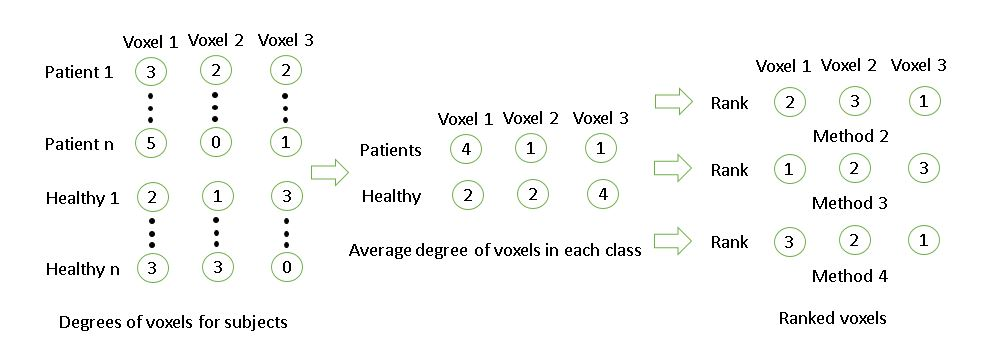
\includegraphics[width=\textwidth]{diagrams/Voxel_ranking.jpg}
\caption{Voxel ranking methods to select best voxels, method 2 ranks the voxels 
based on the absolute difference between the class average degrees,  3 ranks 
based on the difference between the patients average degreees and healthy 
average degrees and method 4 ranks based on the difference between the healthy 
and patients average differences.}
\end{figure}
First, we executed the approach proposed by Rish \emph{et al.}~\cite{Rish_2013} 
on our data set. In the data set we used we had degrees of each voxels as well 
as the smoothed log values of the voxels for each subject. Furthermore, as 
some voxels of some subjects had zero values for the BOLD signal, an universal 
mask was used to select the voxels which had a non-zero BOLD signal value 
through the whole data set. This resulted in a $28719$ voxels per each subject. 
However, using all the available voxels resulted in computation difficulties 
and thus selecting the best voxels (based on the training data) to separate 
the healthy and schizophrenic subjects was very important. 

To select the best voxels out of the possible $28719$ voxels, we experimented multiple approaches. 
These include \begin{enumerate}
  \item Selecting the voxels based on the t-test.
  \item Selecting the voxels based on the absolute differences between the mean degrees of a voxel between schizophrenic and healthy subjects.
  \item Selecting the voxels based on the differences between the mean degrees of a voxel between schizophrenic and healthy subjects.
  \item Selecting the voxels based on the differences between the mean degrees of a voxel between healthy and schizophrenic subjects.
\end{enumerate}
The last three voxel ranking methods are explained in Figure~\ref{fig:voxel_rank}. 
Out of the above four approaches we obtained the highest accuracy on our cross 
validation set by the third approach. Also the number of voxels $k$ to be used 
in the SGMRF model was decided by running the experiment for different $k$ 
values and found the optimum value$20$ for our cross validation set. By using 
the selected voxels, we obtained the precision matrices for schizophrenic and 
healthy subjects. Similar to the value of $k$, the sparsity coefficient 
$\lambda$ was also obtained through a hyperparameter search on our cross 
validation set.

\subsection{SGMRF with degrees from Dorsolateral Prefrontal Cortex area}
connections in certain areas of the brain specifically dorsolateral prefrontal cortex (DLPFC) \cite{Potkin2008} and thalamocortical\cite{Cheng2015} circuitry. Thus, we extracted the degrees of voxels in these areas and used them to build the SGMRF model. Since we had only $4504$ voxels for each subject, we did not perform any voxel rankings in this approach. Similar to the previous approach using the smoothed log values of the degrees resulted in higher accuracy.

\subsection{Methods using Power \emph{et al.}'s ROIs}

The following three methods used in this subsection all involve the $264$  
regions of interest that are described in work by Power \emph{et al.}.
Due to missing data resulting from incomplete scans of subjects, $8$
regions were removed from analysis leaving $256$ ROIs. The regions removed
are characterized by region number with the associated MNI coordinates 
described in Power \emph{et al.} provided in parenthesis: 81 (-44, 12, -34), 
82 (46, 16, -30), 128 (52, 7, -30), 184 (17, -80, -34), 247 (33, 12, -34), 
248 (-31, -10, -36), 249 (49, -3, -38) and 250 (-50, -7, -39). We use the
same approach as described by Vega \emph{et al.}~\cite{rvega} to summarize
regions of interest by taking region averages for each of the $5mm$ radius
spheres that define regions. Finally this results in a $137 \times 256$ matrix
for each subject where each row is a time point across all regions and each
column is the average time series for a single region.


\subsubsection{ROI with Subject Concatenation}

For this approach we follow the method as described by Vega \emph{et al.}.
Training set subjects in each class are first concatenated so that two large 
matrices are created, one with dimension $ns * 137 \times 256$ and the other 
with dimension $nh * 137 \times 256$ where $ns$ is the number of schizophenic 
subjects in the training set and $nh$ is the number of health subjects. To
make learning the MRF structure easier, feature normalization is performed
were for each class and each region in that class, the region mean is 
subtracted from each time point and each time point is divided by the 
region standard deviation.

\begin{equation}
ClassRegion_i = \frac{ClassRegion_i - mean(ClassRegion_i)}{std(ClassRegion_i)}
\end{equation}

Next, with the use of GLasso, a SGMRF structure is learned for each class 
which results in two sparse precision matrices that encode the independences
learned. 

Finally, when presented with a new subject from the hold-out set, the equation
below is used to determine the likelihood of the subject belonging to each
class. The class with the highest likelihood then becomes the predicted label
for the subject.

A modified version of this approach was also implemented and tested but has
been omitted for brevity and due to it obtaining poor results. In this variant
a Fourier transform was used on each of the subject's time series data to 
obtain Fourier coefficients. These Fourier coefficients were then used in 
place of the original time series for learning a classifier.

\begin{equation}
insert here
\end{equation}

%\subsubsection{ROI with Fouier Coefficients}

\subsubsection{Region Degrees and SVMs}

Like the work described in Rish \emph{et al.} region degrees are also used in
this approach but in this case, we only consider the degrees that result from
the $256$ ROIs. This process is illustrated in Figure!\ref{}. For each subject 
we generate a correlation matrix that records the correlation between the 
average time series in their $region_i$ and $region_j$. Because we are not 
interested in the correlation between a region and itself (which is trivially 
$1$) we subtract the diagonal of the correlation matrix from itself. Using a
threshold of $0.7$ which was chosen based on work by Rish \emph{et al.}, we
then proceed to create the binary matrix and sum the column values as 
described previously.

\begin{figure}[!htb]
  \centering
  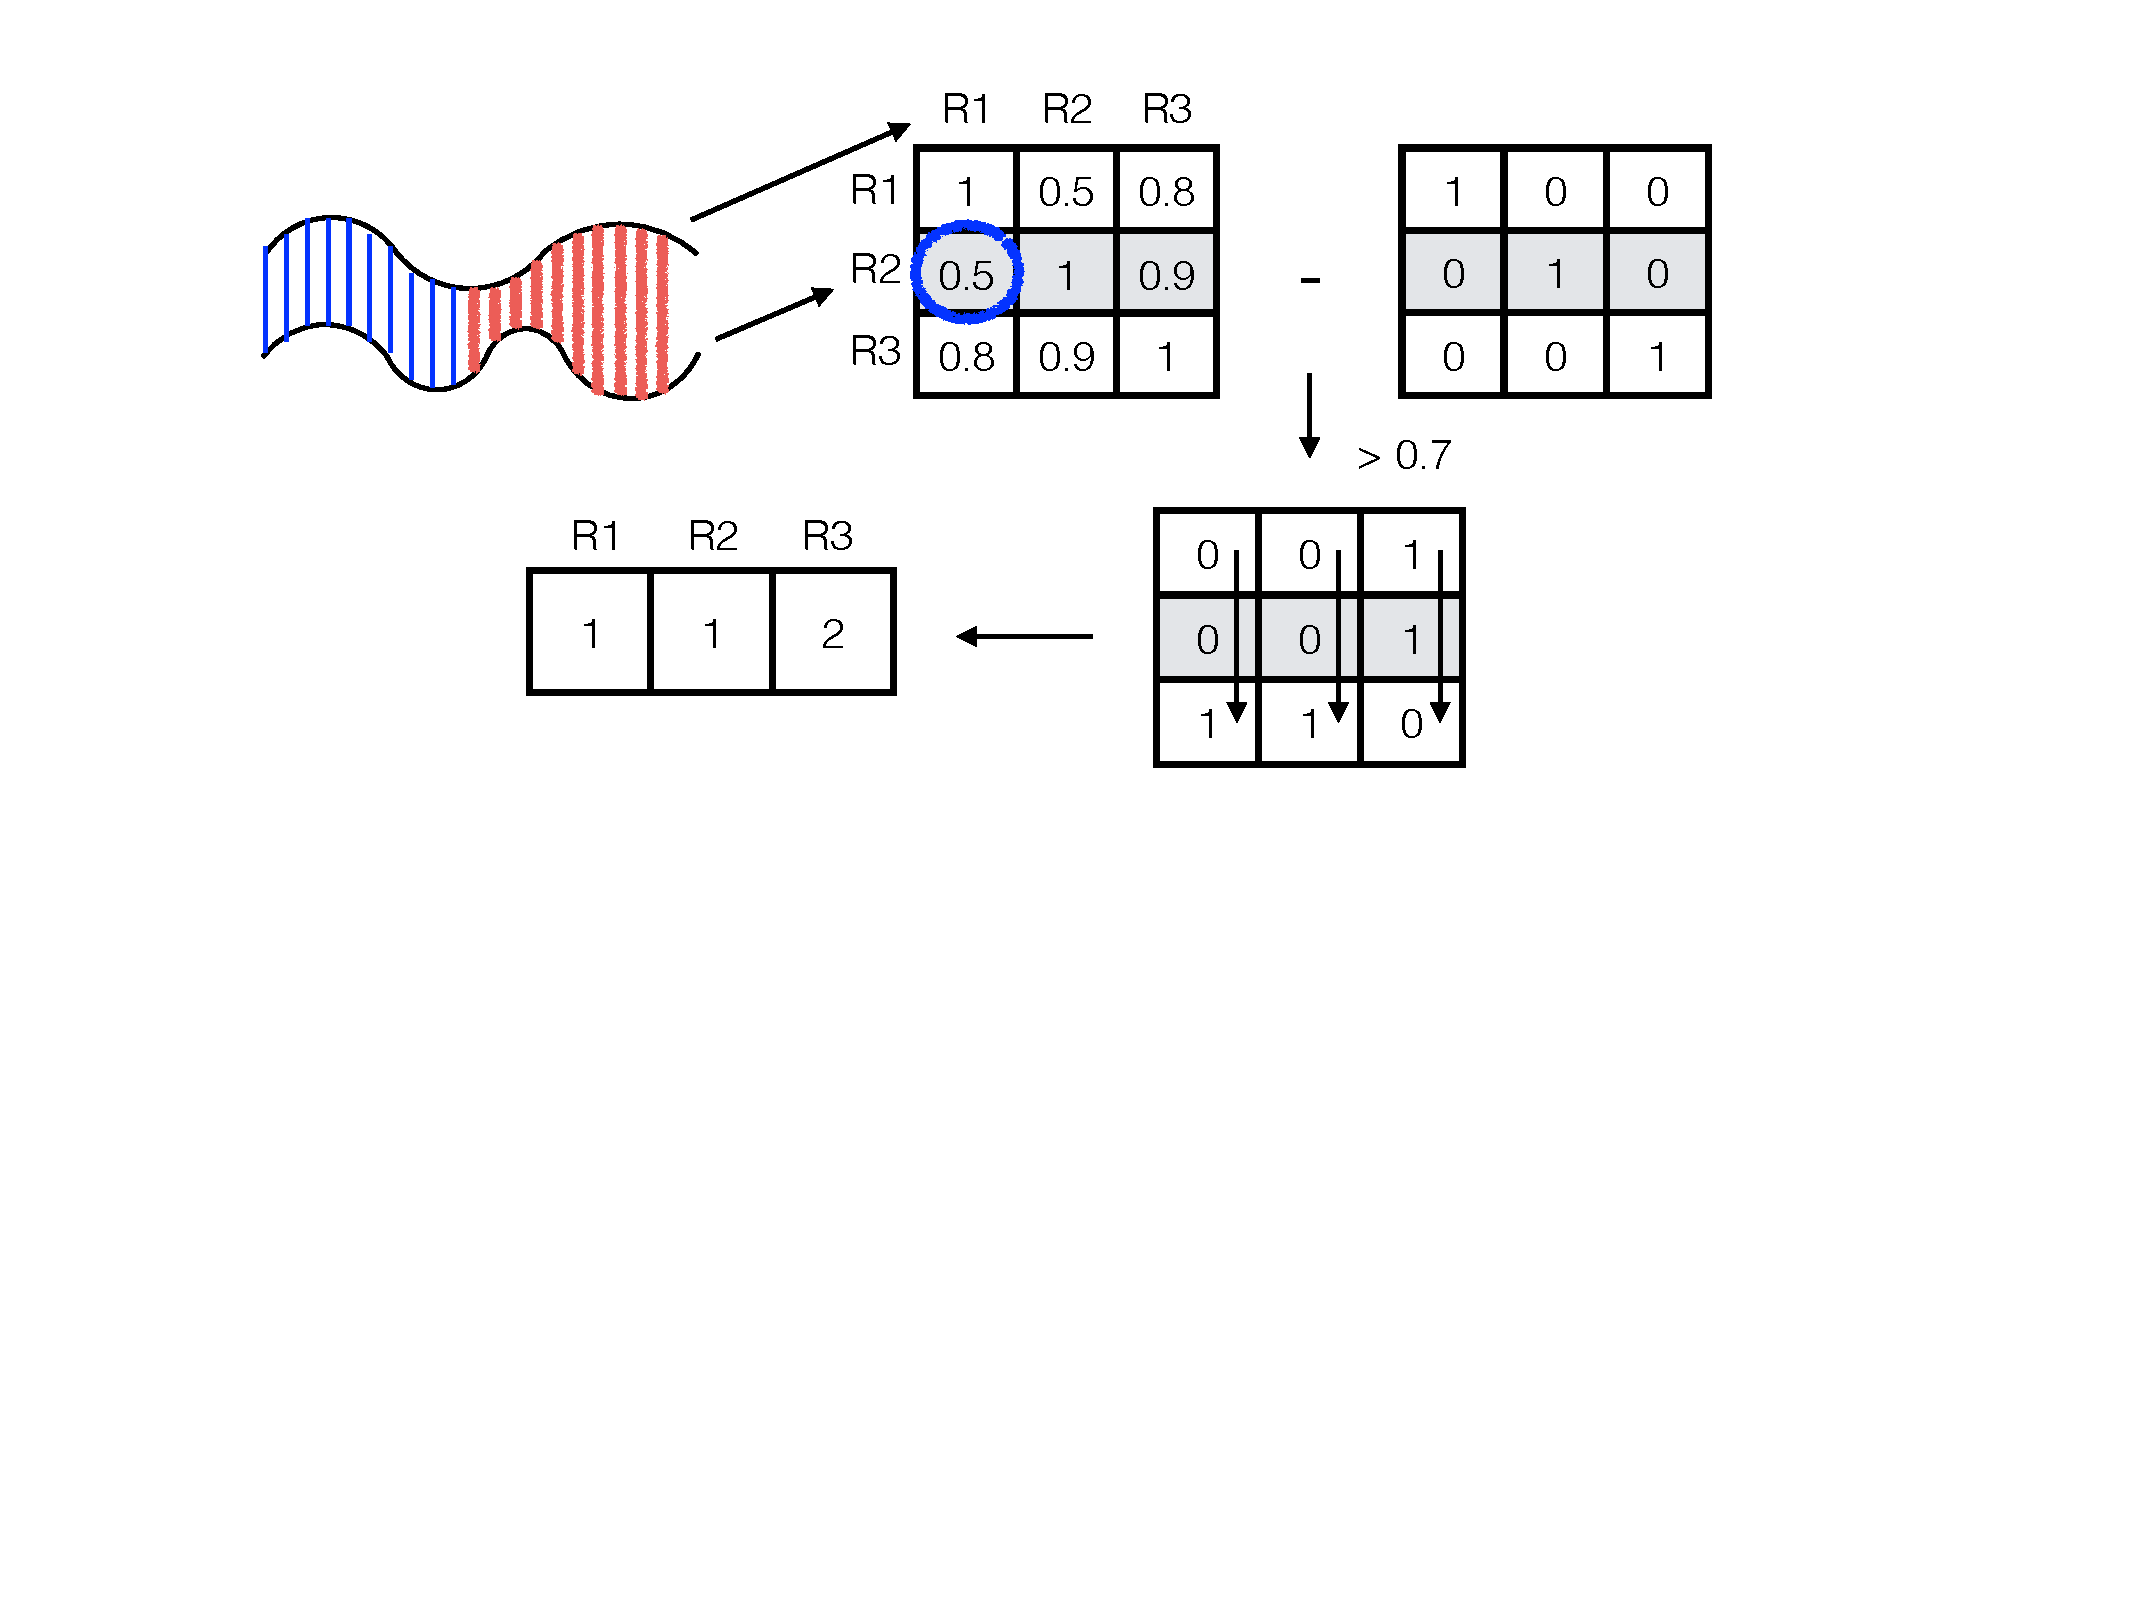
\includegraphics[width=\textwidth, height=5.5cm]{diagrams/ROI_deg_img.pdf}
  \caption{Pair-wise comparisons are made between region time series data to
  produce a correlation matrix. The diagonal is removed and a threshold is
  applied to binarize the matrix. Sums are collected for each region to
  produce the ``degree'' of that region.}
  \label{fig:degree_calc}
\end{figure}

Now that we have a vector of region degrees ($1 \times 256$) for each subject,
a SGMRF is used to again to build a classifier. This follows similarly from
the previous approach except that now the input to GLasso is a $ns \times 256$
matrix for schizophrenic patients and a $nh \times256$ matrix for healthy
subjects. Again this results in two $256 \times 256$ precision matrices which
we can use in likelihood calculations for subjects from the hold-out set.

Additionally, we also used a linear SVM classifier trained directly on
region degree data to compare its performance to the SGMRF classifier.

\subsubsection{Individual MRF Structure Classification}
This approach is similar to the region concatenation approach described 
previously except that here we do not concatenate subjects and instead
learn a precision matrix (sparse MRF structure) for each subject 
individually. For example, if we have $ns_{total}$ schizophrenics in our 
dataset and $nh_{total}$ healthy subjects ($ns_{total} + nh_{total}$ 
$137 \times 256$ matrices) then we will use GLasso to generate $ns + nh$ 
precision matrices.

To build a classifier, a linear SVM is trained on the precision matrices 
generated from the training set and then tested on the precision matrices 
generated from the hold-out set.

\subsection{Your Approach? Farhad}
Describe your experiments


\section{Results}

\begin{table*}[!htb]\footnotesize
\begin{center}
    \begin{tabular}{| l | r | r | r | r | r | r |}
    \hline
                & Rish (Full) & Rish (DLPFC) & ROI + Concatenation & Region Degrees & MRF structure & PCA \\ \hline
    Classifier  & SGMRF       & SGMRF        & SGMRF               & SVM            & SVM           &1    \\ \hline
    Accuracy    & 72.32\%     & 63.52\%      & 74.17               & 60.65          & 69.44         &1    \\ \hline
    \end{tabular}
    \caption{Accuracy on 5 Striated Hold-out Sets}
     \label{fig:holdout_table}
\end{center}
\end{table*}

\section{Discussion}
% this needs to be a well thought out section
% We do we get the results we do, explain this

\section{Conclusions and Future Work}
% General conclusions and restatement of discussion

\section{Acknowledgements}
We would like to thank Dr. Mina Gheiratmand for preprocessing the fMRI data 
and co-coaching our project. Also we used the feature extraction codes 
provided by Dr. Irina Rish.

\bibliographystyle{plain}
\bibliography{T4_Report}

	
\end{document}
